\documentclass[t,usenames,dvipsnames]{beamer}
\usetheme{Copenhagen}
\setbeamertemplate{headline}{} % remove toc from headers
\beamertemplatenavigationsymbolsempty

\usepackage{amsmath, tikz, xcolor, array, graphicx, pgf, pgfplots, standalone}
\pgfplotsset{compat=newest}
\usetikzlibrary{arrows.meta}
\everymath{\displaystyle}

\title{Properties of Functions}
\author{}
\date{}

\AtBeginSection[]
{
  \begin{frame}
    \frametitle{Objectives}
    \tableofcontents[currentsection]
  \end{frame}
}

\begin{document}

\begin{frame}
    \titlepage
\end{frame}


\section{Determine increasing, decreasing, and constant intervals of a function}

\begin{frame}{Increasing Intervals}
A function is \alert{increasing} in an interval if the $y$-coordinates increase in value as the $x$-coordinates increase in value.    \newline\\   \pause

\begin{itemize}
    \item Visually, the graph is moving ``upward" from left to right.   \newline\\  \pause
    \item ``Machine-wise," the outputs go up in value as the inputs go up in value. \newline\\  \pause
    \item Mathematically, if $a < b$ then $f(a) < f(b)$.    \newline\\  \pause
\end{itemize}

\begin{center}
    {\color{red}\textbf{***FOCUS ON THE X-COORDINATES***}}
\end{center}
\end{frame}

\begin{frame}{Decreasing Intervals}
A function is \alert{decreasing} in an interval if the $y$-coordinates decrease in value as the $x$-coordinates increase in value.  \newline\\  \pause

\begin{itemize}
    \item Visually, the graph is moving ``downward" from left to right.   \newline\\  \pause
    \item ``Machine-wise," the outputs go down in value as the inputs go up in value. \newline\\  \pause
    \item Mathematically, if $a < b$ then $f(a) > f(b)$.    \newline\\  \pause
\end{itemize}

\begin{center}
    {\color{red}\textbf{***FOCUS ON THE X-COORDINATES***}}
\end{center}
\end{frame}


\begin{frame}{Constant Intervals}
A function is \alert{constant} in an interval if the $y$-coordinates do not change in value as the $x$-coordinates increase in value.  \newline\\  \pause

\begin{itemize}
    \item Visually, the graph is a horizontal line.   \newline\\  \pause
    \item ``Machine-wise," the outputs don't change as the inputs go up in value. \newline\\  \pause
    \item Mathematically, $f(a) = f(b)$ for all $a$ and $b$ in the interval.    \newline\\  \pause
\end{itemize}

\begin{center}
    {\color{red}\textbf{***FOCUS ON THE X-COORDINATES***}}
\end{center}
\end{frame}

\begin{frame}{Example 1}
Determine the intervals in which the function is increasing, decreasing, and constant.   \newline\\
\begin{minipage}{0.6\textwidth}
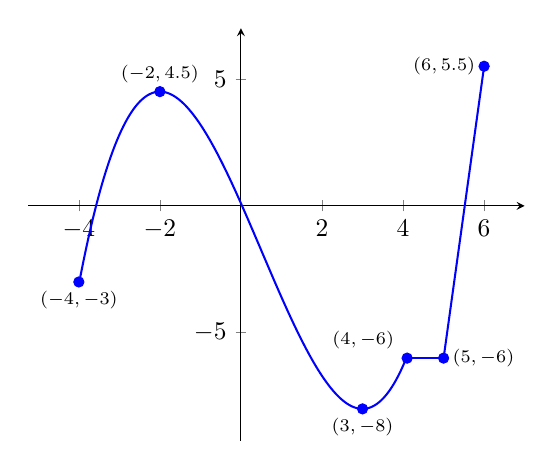
\begin{tikzpicture}[scale=0.92]
\begin{axis}[
axis lines = middle,
xmin = -5.25, xmax = 7,
ymin = -9.25, ymax = 7
]
\addplot [mark = *, only marks,blue] coordinates {(-4,-3) (-2,4.5) (3,-8) (4.1,-6) (5,-6) (6,5.5)};
\addplot [domain=-4:4.1, samples=200,smooth, thick, blue] {(2*x^3-3*x^2-36*x+1)/10};
\addplot [domain=4:5, thick, blue] {-6};
\draw[thick, blue] (axis cs: 5,-6) -- (axis cs: 6,5.5);
\node at (axis cs: -4,-3) [below] {\scriptsize $(-4,-3)$};
\node at (axis cs: -2,4.5) [above] {\scriptsize $(-2,4.5)$};
\node at (axis cs: 3,-8) [below] {\scriptsize $(3,-8)$};
\node at (axis cs: 4,-6) [above left] {\scriptsize $(4,-6)$};
\node at (axis cs: 5,-6) [right] {\scriptsize $(5,-6)$};
\node at (axis cs: 6,5.5) [left] {\scriptsize $(6,5.5)$};
\end{axis}
\end{tikzpicture}
\end{minipage}
\hspace{-0.23cm}
\begin{minipage}{0.4\textwidth}
\onslide<2->{\textbf{Increasing:}} \\\\
\onslide<3->{$(-4,-2)\cup(3,4)\cup(5,6)$}   \\\\
\onslide<4->{\textbf{Decreasing:}} \\\\
\onslide<5->{$(-2,3)$} \\\\
\onslide<6->{\textbf{Constant:}} \\\\
\onslide<7->{$(4,5)$}
\end{minipage}
\end{frame}


\section{Determine relative (local) maximum and minimum coordinates}


\begin{frame}{Relative Maximum}
A \alert{relative (or local) maximum} is the highest point in some interval. \newline\\  \pause
\begin{itemize}
    \item It is a ``top of the hill" for many functions.  \newline\\  \pause
    \item Where the graph \underline{changes from increasing to decreasing}.  \newline\\  \pause
\end{itemize}

An absolute, or global, maximum is the highest point in the entire domain of the function.  \newline\\  \pause

\textbf{{\color{red}***GIVE YOUR ANSWER AS AN ORDERED PAIR***}}
\end{frame}


\begin{frame}{Relative Minimum}
A \alert{relative (or local) minimum} is the lowest point in some interval. \newline\\  \pause
\begin{itemize}
    \item It is a ``bottom of the valley" for many functions.  \newline\\  \pause
    \item Where the graph \underline{changes from decreasing to increasing}.  \newline\\  \pause
\end{itemize}

An absolute, or global, minimum is the lowest point in the entire domain of the function.  \newline\\  \pause

\textbf{{\color{red}***GIVE YOUR ANSWER AS AN ORDERED PAIR***}}
\end{frame}

\begin{frame}{Example 2}
Determine the relative minimum and relative maximum for each. Then determine the global minimum and global maximum.    \newline\\
\begin{minipage}{0.585\textwidth}
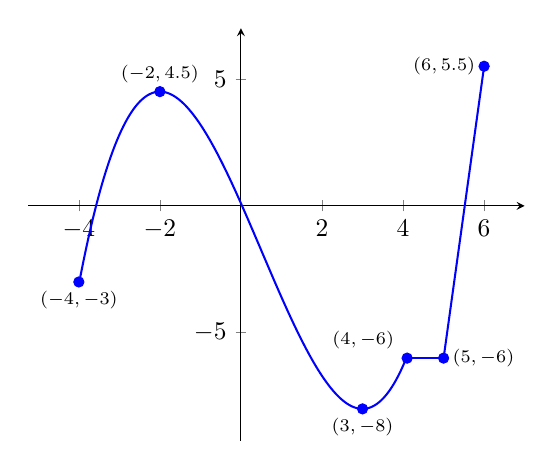
\begin{tikzpicture}[scale=0.92]
\begin{axis}[
axis lines = middle,
xmin = -5.25, xmax = 7,
ymin = -9.25, ymax = 7
]
\addplot [mark = *, only marks,blue] coordinates {(-4,-3) (-2,4.5) (3,-8) (4.1,-6) (5,-6) (6,5.5)};
\addplot [domain=-4:4.1, samples=200,smooth, thick, blue] {(2*x^3-3*x^2-36*x+1)/10};
\addplot [domain=4:5, thick, blue] {-6};
\draw[thick, blue] (axis cs: 5,-6) -- (axis cs: 6,5.5);
\node at (axis cs: -4,-3) [below] {\scriptsize $(-4,-3)$};
\node at (axis cs: -2,4.5) [above] {\scriptsize $(-2,4.5)$};
\node at (axis cs: 3,-8) [below] {\scriptsize $(3,-8)$};
\node at (axis cs: 4,-6) [above left] {\scriptsize $(4,-6)$};
\node at (axis cs: 5,-6) [right] {\scriptsize $(5,-6)$};
\node at (axis cs: 6,5.5) [left] {\scriptsize $(6,5.5)$};
\end{axis}
\end{tikzpicture}
\end{minipage}
\hspace{-0.1cm}
\begin{minipage}{0.4\textwidth}
\onslide<2->{\textbf{Relative Minimum}} \\
\onslide<3->{$(3,-8)$}   \\\\
\onslide<4->{\textbf{Relative Maximum:}} \\
\onslide<5->{$(-2,4.5)$} \\\\
\onslide<6->{\textbf{Global Minimum:}} \\
\onslide<7->{$(3,-8)$}   \\\\
\onslide<8->{\textbf{Global Maximum:}}  \\
\onslide<9->{$(6,5.5)$}
\end{minipage}
\end{frame}

\section{Determine if a function is even or odd}

\begin{frame}{Even Functions}
A function $f$ is \alert{even} if
\[  f(-x) = f(x) \]
\pause

Negative input values give you the same outputs as their positive opposites. \newline\\    \pause

Even functions are symmetric with respect to the $y$-axis.
\end{frame}

\begin{frame}{Odd Functions}
A function $f$ is \alert{odd} if
\[  f(-x) = -f(x) \]
\pause

Negative input values give you the opposite outputs as their positive opposites. \newline\\    \pause

Odd functions are symmetric with respect to the origin.
\end{frame}

\begin{frame}{Example 3}
Determine whether each of the following functions is even, odd, or neither.  \newline\\
(a) \quad $f(x) = \dfrac{5}{2-x^2}$
\begin{align*}
    \onslide<2->{f(-x) &= \frac{5}{2-(-x)^2}} \\[10pt]
    \onslide<3->{&= \frac{5}{2-x^2}} \\[10pt]
    \onslide<4->{&= f(x)}
\end{align*}

\onslide<5->{$f(x) = \dfrac{5}{2-x^2}$ is even}
\end{frame}


\begin{frame}{Example 3}
(b) \quad $g(x) = \dfrac{5x}{2-x^2}$
\begin{align*}
    \onslide<2->{g(-x) &= \frac{5(-x)}{2-(-x)^2}} \\[10pt]
    \onslide<3->{&= \frac{-5x}{2-x^2}} \\[10pt]
    \onslide<4->{&= -\left(\frac{5x}{2-x^2}\right)} \\[10pt]
    \onslide<5->{&= -g(x)}
\end{align*}

\onslide<6->{$g(x) = \dfrac{5x}{2-x^2}$ is odd}
\end{frame}

\begin{frame}{Example 3}
(c) \quad $h(x) = \frac{5x}{2-x^3}$
\begin{align*}
    \onslide<2->{h(-x) &= \frac{5(-x)}{2-(-x)^3}}   \\[10pt]
    \onslide<3->{&= \frac{-5x}{2+x^3}} \\[10pt]
    \onslide<4->{&= -\left(\frac{5x}{2+x^3}\right)} 
\end{align*}

\onslide<5->{$h(x) = \dfrac{5x}{2-x^3}$ is neither odd nor even}
\end{frame}


\begin{frame}{Example 3}
(d) \quad $i(x) = \dfrac{5x}{2x-x^3}$
\begin{align*}
    \onslide<2->{i(-x) &= \frac{5(-x)}{2(-x)-(-x)^3}}   \\[10pt]
    \onslide<3->{&= \frac{-5x}{-2x+x^3}} \\[10pt]
    \onslide<4->{&= \frac{-5x}{-1(2x-x^3)}}    \\[10pt]
    \onslide<5->{&= \frac{5x}{2x-x^3}} \\[10pt]
    \onslide<6->{&= i(x)}
\end{align*}
\end{frame}


\begin{frame}{Example 3}
(e) \quad $j(x) = x^2 - \frac{x}{100} - 1$
\begin{align*}
    \onslide<2->{j(-x) &= (-x)^2 - \frac{-x}{100} - 1} \\[10pt]
    \onslide<3->{&= x^2 + \frac{x}{100} - 1}
\end{align*}

\onslide<4->{$j(x)$ is neither odd nor even.}
\end{frame}

\begin{frame}{Example 4}
Given the graph of $y=f(x)$, find each. \newline\\
\begin{minipage}{0.6\textwidth}
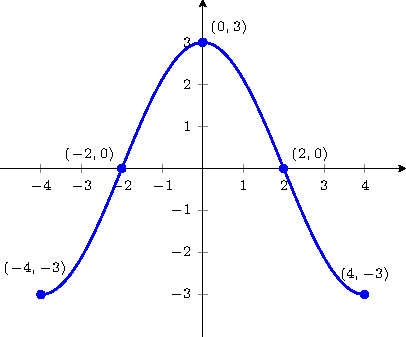
\includegraphics{example4.pdf}
\end{minipage}
\hspace{0.5cm}
\begin{minipage}{0.33\textwidth}
(a) Domain of $f$  \\\\
\onslide<2->{$[-4, 4]$} \\\\
\onslide<3->{(b) Range of $f$} \\\\
\onslide<4->{$[-3,3]$}
\end{minipage}
\end{frame}

\begin{frame}{Example 4}
Given the graph of $y=f(x)$, find each. \newline\\
\begin{minipage}{0.6\textwidth}
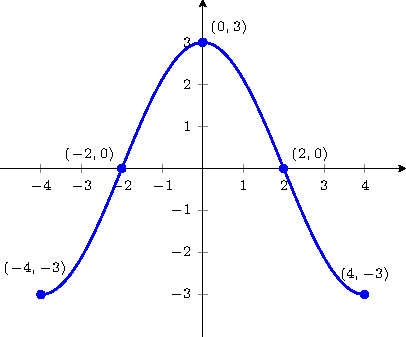
\includegraphics{example4.pdf}
\end{minipage}
\hspace{0.5cm}
\begin{minipage}{0.33\textwidth}
(c) $x$-intercepts  \\\\
\onslide<2->{$(-2,0)\text{ and } (2,0)$} \\\\
\onslide<3->{(d) $y$-intercept} \\\\
\onslide<4->{$(0,3)$}
\end{minipage}
\end{frame}

\begin{frame}{Example 4}
Given the graph of $y=f(x)$, find each. \newline\\
\begin{minipage}{0.6\textwidth}
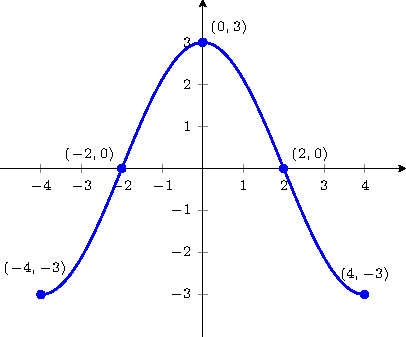
\includegraphics{example4.pdf}
\end{minipage}
\hspace{0.5cm}
\begin{minipage}{0.33\textwidth}
(e) Zeros of $f$  \\\\
\onslide<2->{$(-2,0)\text{ and } (2,0)$} \\\\
\onslide<3->{(f) Solve $f(x)<0$} \\\\
\onslide<4->{$[-4,-2)\cup(2,4]$}
\end{minipage}
\end{frame}

\begin{frame}{Example 4}
Given the graph of $y=f(x)$, find each. \newline\\
\begin{minipage}{0.6\textwidth}
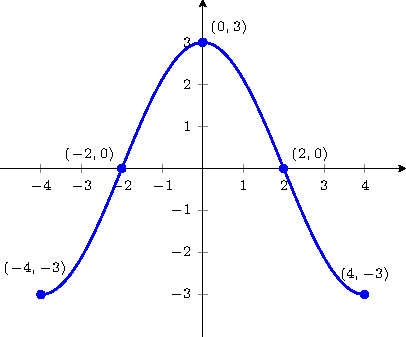
\includegraphics{example4.pdf}
\end{minipage}
\hspace{0.5cm}
\begin{minipage}{0.33\textwidth}
(g) Determine $f(2)$  \\\\
\onslide<2->{0} \\\\
\onslide<3->{(h) Solve $f(x)=-3$} \\\\
\onslide<4->{$x=-4 \text{ and } x=4$}
\end{minipage}
\end{frame}

\begin{frame}{Example 4}
Given the graph of $y=f(x)$, find each. \newline\\
\begin{minipage}{0.6\textwidth}
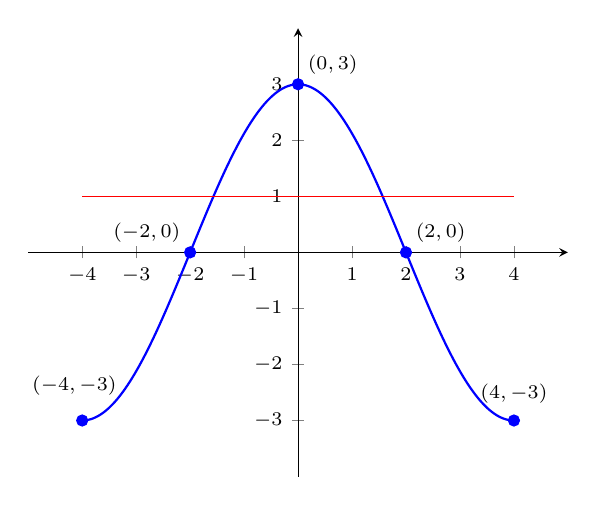
\begin{tikzpicture}[every node/.style={font=\scriptsize}]
\pgfplotsset{every tick label/.append style={font=\scriptsize}}
\begin{axis}[
axis lines = middle,
xmin = -5, xmax = 5,
ymin = -4, ymax = 4,
xtick = {-4,-3,...,4},
ytick = {-3,-2,...,3}
]
\addplot [thick, blue, domain=-4:4, samples=200, smooth] {3*cos(deg(0.785398*x))};
\addplot [color=blue, mark=*, only marks] coordinates {(-4,-3) (-2,0) (0,3) (2,0) (4,-3)};
\node at (axis cs: -4,-3) [above,yshift=0.2cm,xshift=-0.1cm] {$(-4,-3)$};
\node at (axis cs: -2,0) [above left] {$(-2,0)$};
\node at (axis cs: 0,3) [above right] {$(0,3)$};
\node at (axis cs: 2,0) [above right] {$(2,0)$};
\node at (axis cs: 4,-3) [above, yshift=0.1cm] {$(4,-3)$};
\onslide<2->{\addplot[color=red, domain=-4:4] {1};}
\end{axis}
\end{tikzpicture}
\end{minipage}
\hspace{0.5cm}
\begin{minipage}{0.33\textwidth}
(i) Number of solutions to $f(x)=1$  \\\\
\onslide<3->{2} \\\\
\onslide<4->{(j) Does $f$ appear even, odd, or neither?} \\\\
\onslide<5->{even}
\end{minipage}
\end{frame}

\begin{frame}{Example 4}
Given the graph of $y=f(x)$, find each. \newline\\
\begin{minipage}{0.6\textwidth}
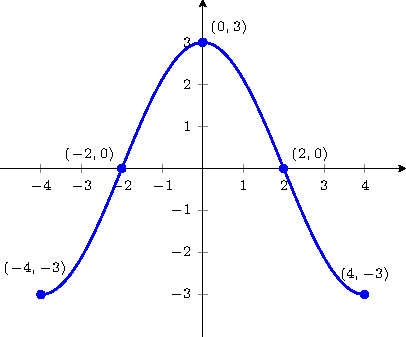
\includegraphics{example4.pdf}
\end{minipage}
\hspace{0.5cm}
\begin{minipage}{0.33\textwidth}
(k) List intervals of increasing and decreasing.  \\\\
\onslide<2->{Increasing:} \\\\
\onslide<3->{$(-4,0)$} \\\\
\onslide<4->{Decreasing:} \\\\
\onslide<5->{$(0,4)$}
\end{minipage}
\end{frame}


\section{Evaluate piecewise-defined functions}


\begin{frame}{Piecewise-Defined Functions}
Piecewise-defined functions take pieces of other functions and put them together (a la Frankenstein).  
\[
f(x) = \begin{cases}
\sin(x-1) + 2 &\text{ if } -9\leq x < -2 \\
x^2 - 3 &\text{ if } -2 \leq x \leq 3 \\
-8x+30 &\text{ if } 3 < x < 4.5\\
\end{cases}
\]
\end{frame}

\begin{frame}{Piecewise-Defined Functions}
\begin{center}
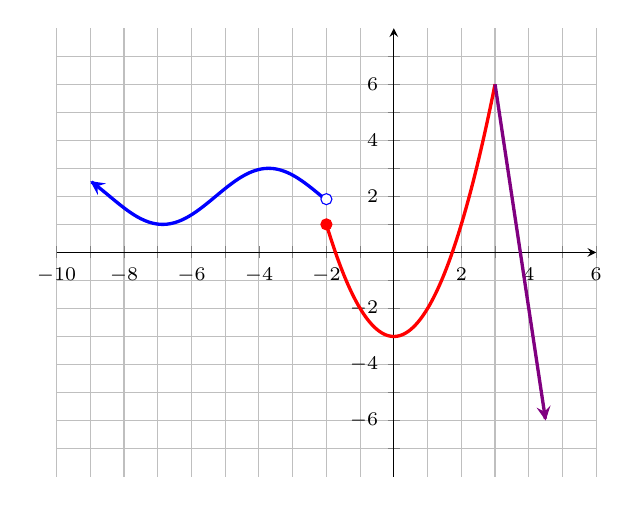
\begin{tikzpicture}[>=stealth, every node/.style = {font=\scriptsize}]
\begin{axis}[
axis lines = middle,
grid,
xmin = -10, xmax = 6,
ymin = -8, ymax = 8,
xtick = {-10,-9,...,10},
xticklabels = {$-10$,,$-8$,,$-6$,,$-4$,,$-2$,,0,,2,,4,,6,,8,,10},
ytick = {-7,-6,...,7},
yticklabels = {,$-6$,,$-4$,,$-2$,,0,,2,,4,,6}
]
\addplot[<-, color=blue, very thick, domain=-9:-2, samples=200,smooth] {sin(deg(x-1))+2};
\addplot[color=red, very thick, domain=-2:3, samples=200,smooth] {x^2-3};
\addplot[->, color=violet, very thick, domain=3:4.5, samples=200, smooth] {-8*x+30};
\draw[color=blue,fill=white] (axis cs:-2,1.9) circle [radius=2pt];
\draw[fill=red,color=red] (axis cs:-2,1) circle [radius=2pt];
\end{axis}
\end{tikzpicture}
\end{center}
\end{frame}

\begin{frame}{Piecewise-Defined Functions}
When evaluating piecewise-defined functions, pay attention to the \alert{domain} of each piece.
\end{frame}

\begin{frame}{Example 5}
Evaulate each for   \newline\\
\begin{minipage}{0.5\textwidth}
\[
f(x) = \begin{cases}
4-x^2 &\text{ if } x < 1 \\
x-3 &\text{ if } x \geq 1 \\
\end{cases}
\]
\end{minipage}
\begin{minipage}{0.4\textwidth}
\begin{align*}
    &\text{(a)} \quad f(-3) \onslide<2->{= -5} \\[15pt]
    &\onslide<3->{\text{(b)} \quad f(0)}
    \onslide<4->{= 4} \\[15pt]
    &\onslide<5->{\text{(c)} \quad f(2)}
    \onslide<6->{=-1} \\[15pt]
    &\onslide<7->{\text{(d)} \quad f\left(\frac{3}{2}\right)}
    \onslide<8->{=-\frac{3}{2}}
\end{align*}
\end{minipage}
\end{frame}



\end{document}
